\documentclass[]{../common/elementary-physics}

\title{3. Mechanical-Electrical Analogies}
\date{2015-05-23 v0.9}

\begin{document}

\maketitle

\tableofcontents

\section{Abstract}

By studying differential equations of damped harmonic oscillators a template is proposed to enable analogies between different systems like mechanical and electrical systems.
Although any linear system that fits the template can be analysed and compared to any other system that fits the template only mass-damper-spring and inductor-resistor-capacitor will be used as examples.

\section{Clues}

In school we are presented formulas for energy such as:

\begin{subequations}
\begin{align}
E &= \frac{m v^2}{2} \tag{kinetic energy} \\
E &= \frac{k x^2}{2} \tag{spring energy} \\
E &= \frac{L I^2}{2} \tag{inductor energy} \\
E &= \frac{C V^2}{2} \tag{capacitor energy}
\end{align}
\end{subequations}

It is hard not to recognize a pattern.
We are also presented formulas such as:

\begin{subequations}
\begin{align}
p &= m v \tag{momentum} \\
F &= k x \tag{spring force} \\
\Lambda &= L I \tag{inductance} \\
Q &= C V \tag{capacitance}
\end{align}
\end{subequations}

where $\Lambda = \Phi N$.
Surely there must be a way to standardize this? 
In the next sections a template and its inverse will be presented, then the template will be applied on LRC,mbk,CRL and kbm systems:

\begin{figure}[ht] \centering
	\subfloat[LRC]
		{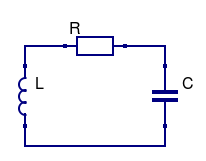
\includegraphics[scale=.5]{LRC} \label{sf1}}
	\subfloat[mbk]
		{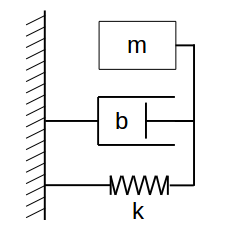
\includegraphics[scale=.3]{mbk} \label{sf3}}
	\subfloat[CRL]
		{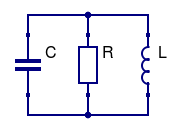
\includegraphics[scale=.5]{CRL} \label{sf2}}
	\subfloat[kbm]
		{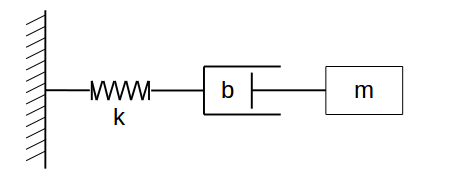
\includegraphics[scale=.3]{kbm} \label{sf4}}
\end{figure}

When other systems are applied to the template we suggest using a spreadsheet to assemble the equations to get it right.

\pagebreak

\section{The Template}

If the oscillator can be described by seven variables $a,b,c,v,x,y$ and $z$ and the equation:

\begin{equation}
a y'' + b y' + c y = 0
\end{equation}

then we can say:

\begin{subequations}
\begin{align}
y &= \int v \, \mathrm{d}t \\
y' &= v \\
y'' &= \frac{\mathrm{d}v}{\mathrm{d}t} \\
f &= \frac{1}{2 \pi \sqrt{\frac{a}{c}}} \tag{frequency} \\
q &= \frac{1}{b} \sqrt{a c} \tag{quality factor}\\
z &= \frac{\mathrm{d}W}{\mathrm{d}y} \\
P &= z v \tag{power} \\
W &= z y = z v t \tag{work} \\
b &= \frac{z}{v} \tag{parasite} \\
P_b &= b v^2 \tag{losses} \\
z = x' &= a \frac{\mathrm{d}v}{\mathrm{d}t} \\
x &= a v \\
E_a &= \frac{a v^2}{2} \tag{energy} \\
z' &= c \frac{\mathrm{d}y}{\mathrm{d}t} \\
z &= c y \\
E_c &= \frac{c y^2}{2} \tag{energy} 
\end{align}
\end{subequations}

Any system that fits the template also has an inverse system.
If the variables are $a,b,c,v,x,y,z$ then the inverse system will have the variables $c^{-1},b^{-1},a^{-1},z,y,x,v$.
One of them can probably be called series and the other parallel.

\pagebreak

\section{LRC-system}

An inductor, resistor and capacitor in series.
All components have the same current, each term is the voltage for the corresponding component.
The sum of the voltages equals zero as in Kirchhoff's second law.
The variables $L,R,C^{-1},I,\Lambda,Q,V$ are used.
$\Lambda = \Phi N$ and is referred to as magnetic flux linkage.

\begin{subequations}
\begin{align}
L Q'' + R Q' + \frac{Q}{C} &= 0 \\
Q &= \int I \, \mathrm{d}t \\
Q' &= I \tag{definition of current} \\
Q'' &= \frac{\mathrm{d}I}{\mathrm{d}t} \\
f &= \frac{1}{2 \pi \sqrt{L C}} \tag{frequency} \\
q &= \frac{1}{R} \sqrt{\frac{L}{C}} \tag{quality factor}\\
V &= \frac{\mathrm{d}W}{\mathrm{d}Q} \\
P &= V I \tag{power} \\
W &= V Q = V I t \tag{work} \\
R &= \frac{V}{I} \tag{Ohm's law} \\
P_R &= R I^2 \tag{losses} \\
V = \Lambda' &= L \frac{\mathrm{d}I}{\mathrm{d}t} \tag{Faraday's law} \\
\Lambda &= L I \tag{definition of inductance} \\
E_L &= \frac{L I^2}{2} \tag{energy in a coil} \\
V' &= \frac{1}{C} \frac{\mathrm{d}Q}{\mathrm{d}t} \\
V &= \frac{Q}{C} \\
E_C &= \frac{Q^2}{2 C} \tag{energy} 
\end{align}
\end{subequations}

\pagebreak

\section{mbk-system}

A mass, damper and spring in series.
All components have the same velocity, each term is the force for the corresponding component.
The sum of the forces equals zero as in Newton's 3rd Law.
The variables $m,b,k,v,p,x,F$ are used.

\begin{subequations}
\begin{align}
m x'' + b x' + k x &= 0 \\
x &= \int v \, \mathrm{d}t \\
x' &= v \tag{definition of velocity} \\
x'' &= \frac{\mathrm{d}v}{\mathrm{d}t} \tag{definition of acceleration} \\
f &= \frac{1}{2 \pi \sqrt{\frac{m}{k}}} \tag{frequency} \\
q &= \frac{\sqrt{m k}}{b} \tag{quality factor}\\
F &= \frac{\mathrm{d}W}{\mathrm{d}x} \\
P &= F v \tag{power} \\
W &= F x = F v t \tag{work} \\
b &= \frac{F}{v} \tag{parasite} \\
P_b &= b v^2 \tag{losses} \\
F = p' &= m \frac{\mathrm{d}v}{\mathrm{d}t} \tag{Newton's 2nd law} \\
p &= m v \tag{definition of momentum} \\
E_m &= \frac{m v^2}{2} \tag{kinetic energy} \\
F' &= k \frac{\mathrm{d}x}{\mathrm{d}t} \\
F &= k x \tag{Hooke's law} \\
E_k &= \frac{k x^2}{2} \tag{energy in a spring} 
\end{align}
\end{subequations}

\pagebreak

\section{CRL-system}

A capacitor, resistor and inductor in parallel.
All components have the same voltage, each term is the current for the corresponding component.
The sum of the currents equals zero as in Kirchhoff's first law.
The variables $C,R^{-1},L^{-1},V,Q,\Lambda,I$ are used.
$\Lambda = \Phi N$ and is referred to as magnetic flux linkage.

\begin{subequations}
\begin{align}
C \Lambda'' + \frac{\Lambda'}{R} + \frac{\Lambda}{L} &= 0 \\
\Lambda &= \int V \, \mathrm{d}t \\
\Lambda' &= V \\
\Lambda'' &= \frac{\mathrm{d}V}{\mathrm{d}t} \\
f &= \frac{1}{2 \pi \sqrt{C L}} \tag{frequency} \\
q &= R \, \sqrt{\frac{C}{L}} \tag{quality factor}\\
I &= \frac{\mathrm{d}W}{\mathrm{d}\Lambda} \\
P &= I V \tag{power} \\
W &= I \Lambda = I V t \tag{work} \\
\frac{1}{R} &= \frac{I}{V} \tag{parasite} \\
P_R &= \frac{V^2}{R} \tag{losses} \\
I = Q' &= C \frac{\mathrm{d}V}{\mathrm{d}t} \\
Q &= C V \tag{definition of capacitance} \\
E_c &= \frac{C V^2}{2} \tag{energy in a capacitor} \\
I' &= \frac{1}{L} \frac{\mathrm{d}\Lambda}{\mathrm{d}t} \\
I &= \frac{\Lambda}{L} \\
E_L &= \frac{\Lambda^2}{2 L} \tag{energy} 
\end{align}
\end{subequations}

\pagebreak

\section{kbm-system}

A spring, damper and mass in parallel.
All components have the same force, each term is the velocity for the corresponding component.
The sum of the velocities equals zero as in common sense.
The variables $k^{-1},b^{-1},m^{-1},F,x,p,v$ are used.

\begin{subequations}
\begin{align}
\frac{p''}{k} + \frac{p'}{b} + \frac{p}{m} &= 0 \\
p &= \int F \, \mathrm{d}t \tag{definition of impulse} \\
p' &= F \\
p'' &= \frac{\mathrm{d}F}{\mathrm{d}t} \\
f &= \frac{1}{2 \pi \sqrt{\frac{m}{k}}} \tag{frequency} \\
q &= \frac{b}{\sqrt{k m}} \tag{quality factor}\\
v &= \frac{\mathrm{d}W}{\mathrm{d}p} \\
P &= v F \tag{power} \\
W &= v p = v F t \tag{work} \\
\frac{1}{b} &= \frac{v}{F} \tag{parasite} \\
P_b &= \frac{F^2}{b} \tag{losses} \\
v = x' &= \frac{1}{k} \frac{\mathrm{d}F}{\mathrm{d}t} \\
x &= \frac{F}{k}\\
E_k &= \frac{F^2}{2 k} \tag{energy} \\
v' &= \frac{1}{m} \frac{\mathrm{d}p}{\mathrm{d}t} \\
v &= \frac{p}{m} \\
E_m &= \frac{p^2}{2 m} \tag{energy} 
\end{align}
\end{subequations}

\pagebreak

\section{Other systems}

Angular velocity-momentum $I,C,\kappa,\omega,L,\theta,\tau$ and it's inverse.

\section{Analogies}

Although the components in $LRC$ and $mbk$ are considered in series and the components in $CRL$ and $kbm$ in parallel any system can be compared to any other:

\begin{center}
\begin{tabular}{c|c|c|c}
\head{LRC} & \head{mbk} & \head{CRL} & \head{kbm} \\
\hline
$L$       & $m$ & $C$       & $k^{-1}$ \\
$R$       & $b$ & $R^{-1}$  & $b^{-1}$ \\
$C^{-1}$  & $k$ & $L^{-1}$  & $m^{-1}$ \\
$I$       & $v$ & $V$       & $F$ \\
$\Lambda$ & $p$ & $Q$       & $x$ \\
$Q$       & $x$ & $\Lambda$ & $p$ \\
$V$       & $F$ & $I$       & $v$
\end{tabular}
\end{center}

In both of our previous papers\cite{ef1ch,ef2ch} we compared $LRC$ to $kbm$.
In the first paper\cite{ef1ch} we had a $LRC$ with two capacitors which added as $C^{-1}_c = C^{-1}_1 + C^{-1}_1$ since the $C$ in $LRC$ is inverted.
We also had a $kbm$ with two masses which also added as $m^{-1}_c = m^{-1}_1 + m^{-1}_1$ since the $m$ in $kbm$ is also inverted.
A more intuitive comparison may be to compare $LRC$ to $mbk$ since both $I$ and $v$ are about movement and both $Q$ and $x$ are stationary.
Which systems you use depends entirely on what you're trying to accomplish by the comparison.

\section{Conclusion}

By using a template like the one proposed it is very easy to transfer knowledge from one harmonic system to another.
This has been proposed by many\cite{wpana} before me but few have included equations like $\Lambda = \Phi N = L I$ and therefore dropped the $N$ only providing $\Phi$ for systems with inductors.

\appendix

\section{In Plain English}

By comparing various harmonic systems and their domain equations we have compiled a general template for all simple harmonic systems.
The variables in the template are replaced by those in the system to be studied and thus can knowledge from one system be transferred to another.
The variables can also be as we call it inverted to obtain a new system.
These two systems, which are each other's inverse, are labelled serial and parallel systems respectively.

\section{På Ren Svenska}

Genom att jämföra olika harmoniska system och deras domäners ekvationer har vi sammanställt en generell schablon för alla enkla harmoniska system.
Variablerna i schablonen byts ut till de i det system man vill studera och på så sätt kan kunskap från ett system överföras till ett annat.
Variablerna kan även som vi kallar det inverteras för att få fram ett nytt system.
Dessa två system, som är varandras invers, kallas för seriellt respektive parallellt system.

\section{This Paper}

This is one paper from a collection of papers, all free to be downloaded and shared. If you have ideas how to enhance any of the papers, if you want to contribute, don’t hesitate to contact us at \url{hob.nilre@gmail.com}.\\
\\
The papers can all be found at:
\begin{itemize}
\item \url{https://sites.google.com/site/nilrehob/home/elementary-physics}
\item \url{https://independent.academia.edu/HobNilre/Papers}
\item \url{https://groups.yahoo.com/neo/groups/EVGRAY/files/Hob/}
\item \url{http://overunity.com/15796/elementary-physics-revisited/}
\item \url{http://idipsum.se/home/elementary%20physics.html}
\item \url{https://github.com/boherlin/elementary-physics/tree/master/pdf}
\end{itemize}

They are updated with new versions in an unpredictable manner, possibly not on all sites but at least on the last two sites in the list, make sure you always have the latest version!
Their \LaTeX source-codes can be found at \url{https://github.com/boherlin/elementary-physics/tree/master/src}.
All papers, but not all versions, have been stamped at \url{http://www.OriginStamp.org}.\\
\\
If you enjoyed this paper, found value in it and want to help us, please consider giving us a donation in bitcoin, this is our address:

\begin{figure}[ht] \centering
	
\includegraphics[]{1B79p75vQw4Rb1GQdmGYpDapFwEytFJDqw} \caption{1B79p75vQw4Rb1GQdmGYpDapFwEytFJDqw}
\end{figure}


\printbibliography

\end{document}

